\documentclass{beamer}
\usepackage[utf8]{inputenc}

\usetheme{Madrid}
\usecolortheme{default}
\usepackage{amsmath,amssymb,amsfonts,amsthm}
\usepackage{txfonts}
\usepackage{tkz-euclide}
\usepackage{listings}
\usepackage{adjustbox}
\usepackage{array}
\usepackage{tabularx}
\usepackage{gvv}
\usepackage{lmodern}
\usepackage{circuitikz}
\usepackage{tikz}
\usepackage{graphicx}
\usepackage{mathtools}

\setbeamertemplate{page number in head/foot}[totalframenumber]

\usepackage{tcolorbox}
\tcbuselibrary{minted,breakable,xparse,skins}



\definecolor{bg}{gray}{0.95}
\DeclareTCBListing{mintedbox}{O{}m!O{}}{%
  breakable=true,
  listing engine=minted,
  listing only,
  minted language=#2,
  minted style=default,
  minted options={%
    linenos,
    gobble=0,
    breaklines=true,
    breakafter=,,
    fontsize=\small,
    numbersep=8pt,
    #1},
  boxsep=0pt,
  left skip=0pt,
  right skip=0pt,
  left=25pt,
  right=0pt,
  top=3pt,
  bottom=3pt,
  arc=5pt,
  leftrule=0pt,
  rightrule=0pt,
  bottomrule=2pt,
  toprule=2pt,
  colback=bg,
  colframe=orange!70,
  enhanced,
  overlay={%
    \begin{tcbclipinterior}
    \fill[orange!20!white] (frame.south west) rectangle ([xshift=20pt]frame.north west);
    \end{tcbclipinterior}},
  #3,
}
\lstset{
    language=C,
    basicstyle=\ttfamily\small,
    keywordstyle=\color{blue},
    stringstyle=\color{orange},
    commentstyle=\color{green!60!black},
    numbers=left,
    numberstyle=\tiny\color{gray},
    breaklines=true,
    showstringspaces=false,
}
\title{8.2.11}
\date{29th September, 2025}
\author{Puni Aditya - EE25BTECH11046}

\begin{document}

\frame{\titlepage}
\begin{frame}{Question}
Find the coordinates of the focus, vertex, eccentricity, axis of the conic section, the equation of the directrix and the length of the latus rectum.
\begin{align*}
    \frac{x^2}{100} + \frac{y^2}{400} = 1
\end{align*}
is \rule{2cm}{0.4pt}.
\end{frame}

\begin{frame}{Theoretical Solution}
We use an affine transformation to convert the conic equation to its standard form.
\begin{align*}
    \vec{x}^\top\vec{V}\vec{x} + 2\vec{u}^\top\vec{x} + f = 0
\end{align*}
The symmetric matrix $\vec{V}$ is spectrally decomposed to align axes with eigenvectors.
\begin{align}
    \vec{V} = \vec{P}\vec{D}\vec{P}^\top, \text{ } \vec{D} = \myvec{\lambda_1 & 0 \\ 0 & \lambda_2}, \text{ } \vec{P}^\top\vec{P} = \vec{I}
\end{align}
\end{frame}

\begin{frame}{Theoretical Solution}
Substituting the decomposition into the conic equation.
\begin{align}
    \vec{x}^\top\vec{P}\vec{D}\vec{P}^\top\vec{x} + 2\vec{u}^\top\vec{x} + f = 0
\end{align}
A rotation
\begin{align}
    \vec{x_r} = \vec{P}^\top\vec{x} 
\end{align}
aligns the conic with the coordinate axes.
\begin{align}
    \vec{x} = \vec{P}\vec{x_r}
\end{align}
\end{frame}

\begin{frame}{Theoretical Solution}
Applying the rotation to the conic equation.
\begin{align}
    \brak{\vec{P}\vec{x_r}}^\top\vec{P}\vec{D}\vec{P}^\top\brak{\vec{P}\vec{x_r}} + 2\vec{u}^\top\brak{\vec{P}\vec{x_r}} + f &= 0 \\
    \vec{x_r}^\top\vec{P}^\top\vec{P}\vec{D}\vec{P}^\top\vec{P}\vec{x_r} + 2\brak{\vec{P}^\top\vec{u}}^\top\vec{x_r} + f &= 0 \\
    \vec{x_r}^\top\vec{D}\vec{x_r} + 2\vec{u_r}^\top\vec{x_r} + f &= 0
\end{align}
\end{frame}

\begin{frame}{Theoretical Solution}
A translation 
\begin{align}
    \vec{x_c} = \vec{x_r} + \vec{D}^{-1}\vec{u_r}
\end{align}
moves the conic's center to the origin.
\begin{align}
    f_c = f - \vec{u_r}^\top\vec{D}^{-1}\vec{u_r}
\end{align}
The center of the conic in the original coordinates is 
\begin{align}
    \vec{c} = -\vec{V}^{-1}\vec{u}
\end{align}
\end{frame}

\begin{frame}{Theoretical Solution}
\begin{align}
    \vec{c} = -\brak{\vec{P}\vec{D}\vec{P}^\top}^{-1}\vec{u} = -\vec{P}\vec{D}^{-1}\vec{P}^\top\vec{u} = -\vec{P}\vec{D}^{-1}\vec{u_r}
\end{align}
The complete transformation from original to centered coordinates is 
\begin{align}
    \vec{x_c} = \vec{P}^\top\brak{\vec{x}-\vec{c}}
\end{align}
\begin{align}
    \vec{x_c} &= \vec{P}^\top\vec{x} + \vec{D}^{-1}\vec{u_r} = \vec{P}^\top\vec{x} - \vec{P}^\top\vec{c} = \vec{P}^\top\brak{\vec{x}-\vec{c}} \\
    \implies \vec{x} &= \vec{P}\vec{x_c} + \vec{c} \label{eq:71}
\end{align}
\end{frame}

\begin{frame}{Theoretical Solution}
The given conic equation
\begin{align}
    \frac{x^2}{100} + \frac{y^2}{400} - 1 = 0
\end{align}
\begin{align}
    \vec{V} = \myvec{\frac{1}{100} & 0 \\ 0 & \frac{1}{400}}, \text{ } \vec{u} = \myvec{0 \\ 0}, \text{ } f = -1
\end{align}
The major axis corresponds to smaller eigenvalue.
\begin{align}
    \lambda_1 = \frac{1}{400}, \text{ } \lambda_2 = \frac{1}{100}, \text{ } \vec{P} = \myvec{0 & 1 \\ 1 & 0}, \text{ } \vec{c} = \myvec{0 \\ 0}
\end{align}
\end{frame}

\begin{frame}{Theoretical Solution}
Applying the rotation to find the canonical coordinates.
\begin{align}
    \vec{x_c} = \vec{P}^\top\vec{x} \implies \myvec{x_c \\ y_c} = \myvec{0 & 1 \\ 1 & 0}\myvec{x \\ y} = \myvec{y \\ x}
\end{align}
The standard form of the ellipse in canonical coordinates.
\begin{align}
    \frac{x_c^2}{-f/\lambda_1} + \frac{y_c^2}{-f/\lambda_2} = 1
\end{align}
\end{frame}

\begin{frame}{Theoretical Solution}
\begin{align}
    e &= \sqrt{1 - \frac{\lambda_1}{\lambda_2}} = \sqrt{1 - \frac{1/400}{1/100}} = \frac{\sqrt{3}}{2} \\
    \vec{f_c} &= \pm\sqrt{\frac{f\brak{\lambda_1 - \lambda_2}}{\lambda_1\lambda_2}}\vec{e_1} = \pm 10\sqrt{3}\vec{e_1} \\
    \vec{v_c} &= \pm\sqrt{\frac{-f}{\lambda_1}}\vec{e_1} = \pm 20\vec{e_1} \\
    \vec{d_c} &: \vec{e_1}^\top\vec{x_c} = \pm\sqrt{\frac{-f\lambda_2}{\lambda_1\brak{\lambda_2-\lambda_1}}} = \pm\frac{40}{\sqrt{3}} \\
    L &= \frac{-2f}{\lambda_2}\sqrt{\frac{\lambda_1}{-f}} = 10
\end{align}
\end{frame}

\begin{frame}{Theoretical Solution}
Transforming properties back to the original coordinate system using \eqref{eq:71}
\begin{align}
    \vec{f} &= \vec{P}\brak{\pm 10\sqrt{3}\vec{e_1}} = \pm 10\sqrt{3}\vec{e_2} \\
    \vec{v} &= \vec{P}\brak{\pm 20\vec{e_1}} = \pm 20\vec{e_2} \\
    \vec{d} &: \vec{e_2}^\top\vec{x} = \pm \frac{40}{\sqrt{3}} \implies \myvec{0 & 1}\vec{x} = \pm \frac{40}{\sqrt{3}}
\end{align}
\end{frame}

\begin{frame}{Theoretical Solution}
\begin{center}
\begin{tabular}{|l|c|}
    \hline
    \textbf{Property} & \textbf{Value} \\
    \hline
    Eccentricity & $\frac{\sqrt{3}}{2}$ \\
    \hline
    Axis & $x=0$ \\
    \hline
    Vertices & $\brak{0, \pm 20}$ \\
    \hline
    Foci & $\brak{0, \pm 10\sqrt{3}}$ \\
    \hline
    Directrices & $y = \pm \frac{40}{\sqrt{3}}$ \\
    \hline
    Latus Rectum & $10$ \\
    \hline
\end{tabular}
\end{center}
\end{frame}

\begin{frame}{Plot}
\begin{figure}
	\centering
	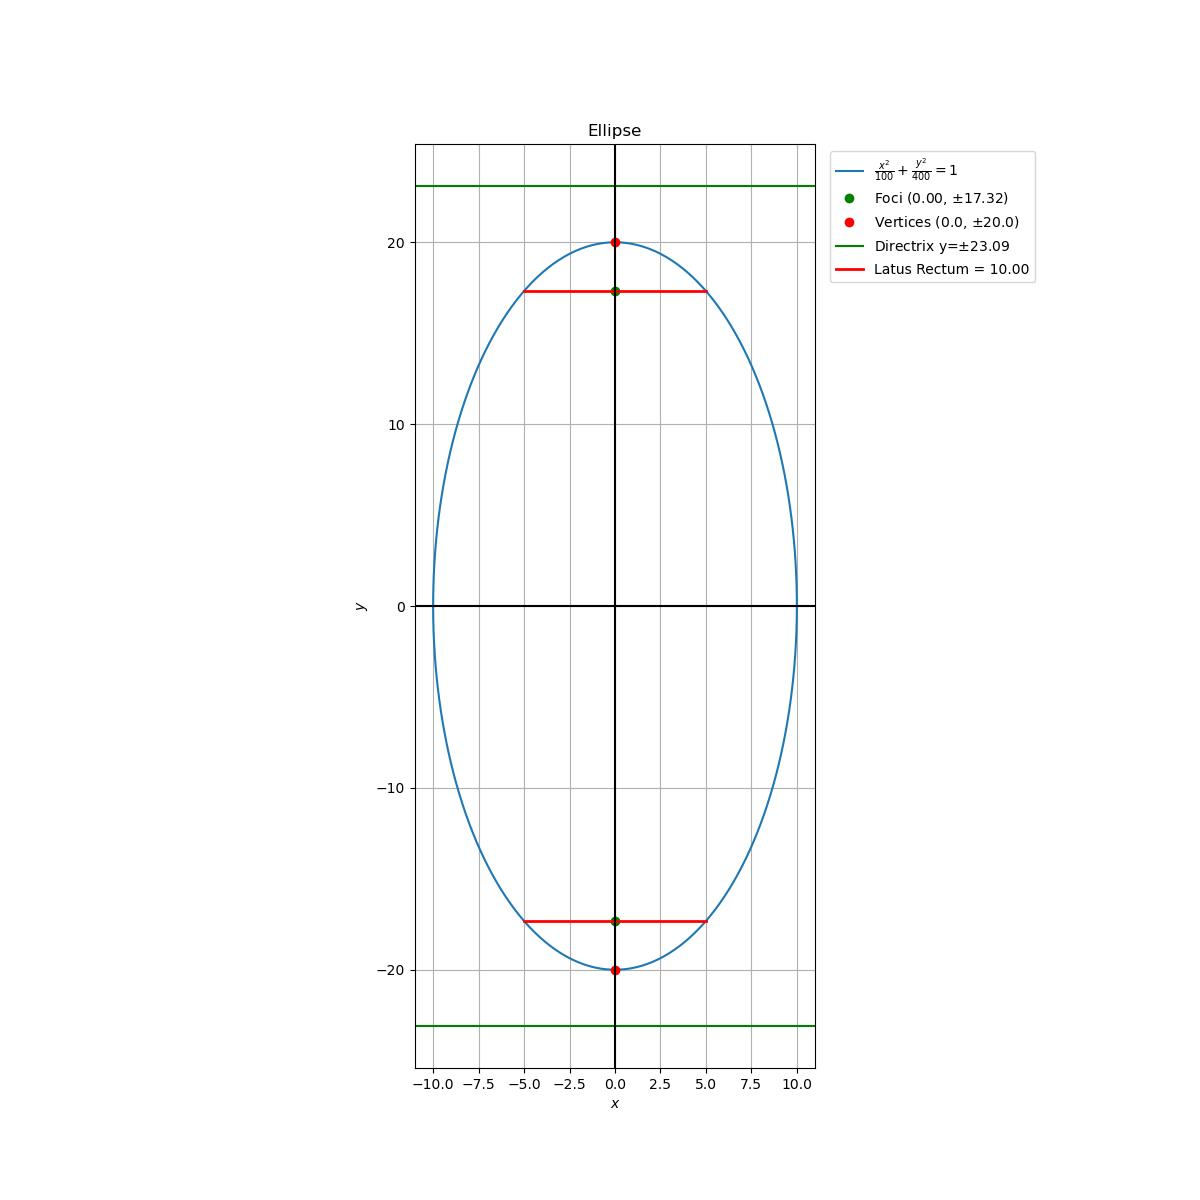
\includegraphics[width=0.5\columnwidth]{../figs/plot_c.jpg}
	\caption{Plot}
	\label{fig:fig}
\end{figure}
\end{frame}

\end{document}
